\section{Introduction}
JavaScript is one of the most widely used programming languages not only for
client-side but also for server-side programming~\cite{nodejs, meanjs} and even
for small embedded systems~\cite{espruino, tessel2}.  It is the top-ranked
language used in active GitHub repositories\footnote{https://githut.info/}, and
\#7 in the TIOBE Programming Community
index\footnote{https://www.tiobe.com/tiobe-index/}.  According to
W3Techs\footnote{https://w3techs.com/technologies/details/cp-javascript/all/all},
95.0\% of websites use JavaScript as their client-side programming language.

Despite its popularity, JavaScript developers often suffer from its intricate
semantics, which may cause unexpected behaviors.  For example, the
following function may seem to always return \( \code{false} \):
\begin{lstlisting}[style=myJSstyle]
        function f(x) { return x == !x; }
\end{lstlisting}
Unfortunately, it returns \( \code{true} \) when its argument
is an empty array \( \code{[]} \).  To correctly understand and reason about
such a complex behavior, the formal semantics of JavaScript is necessary.

\begin{figure}
  \centering
  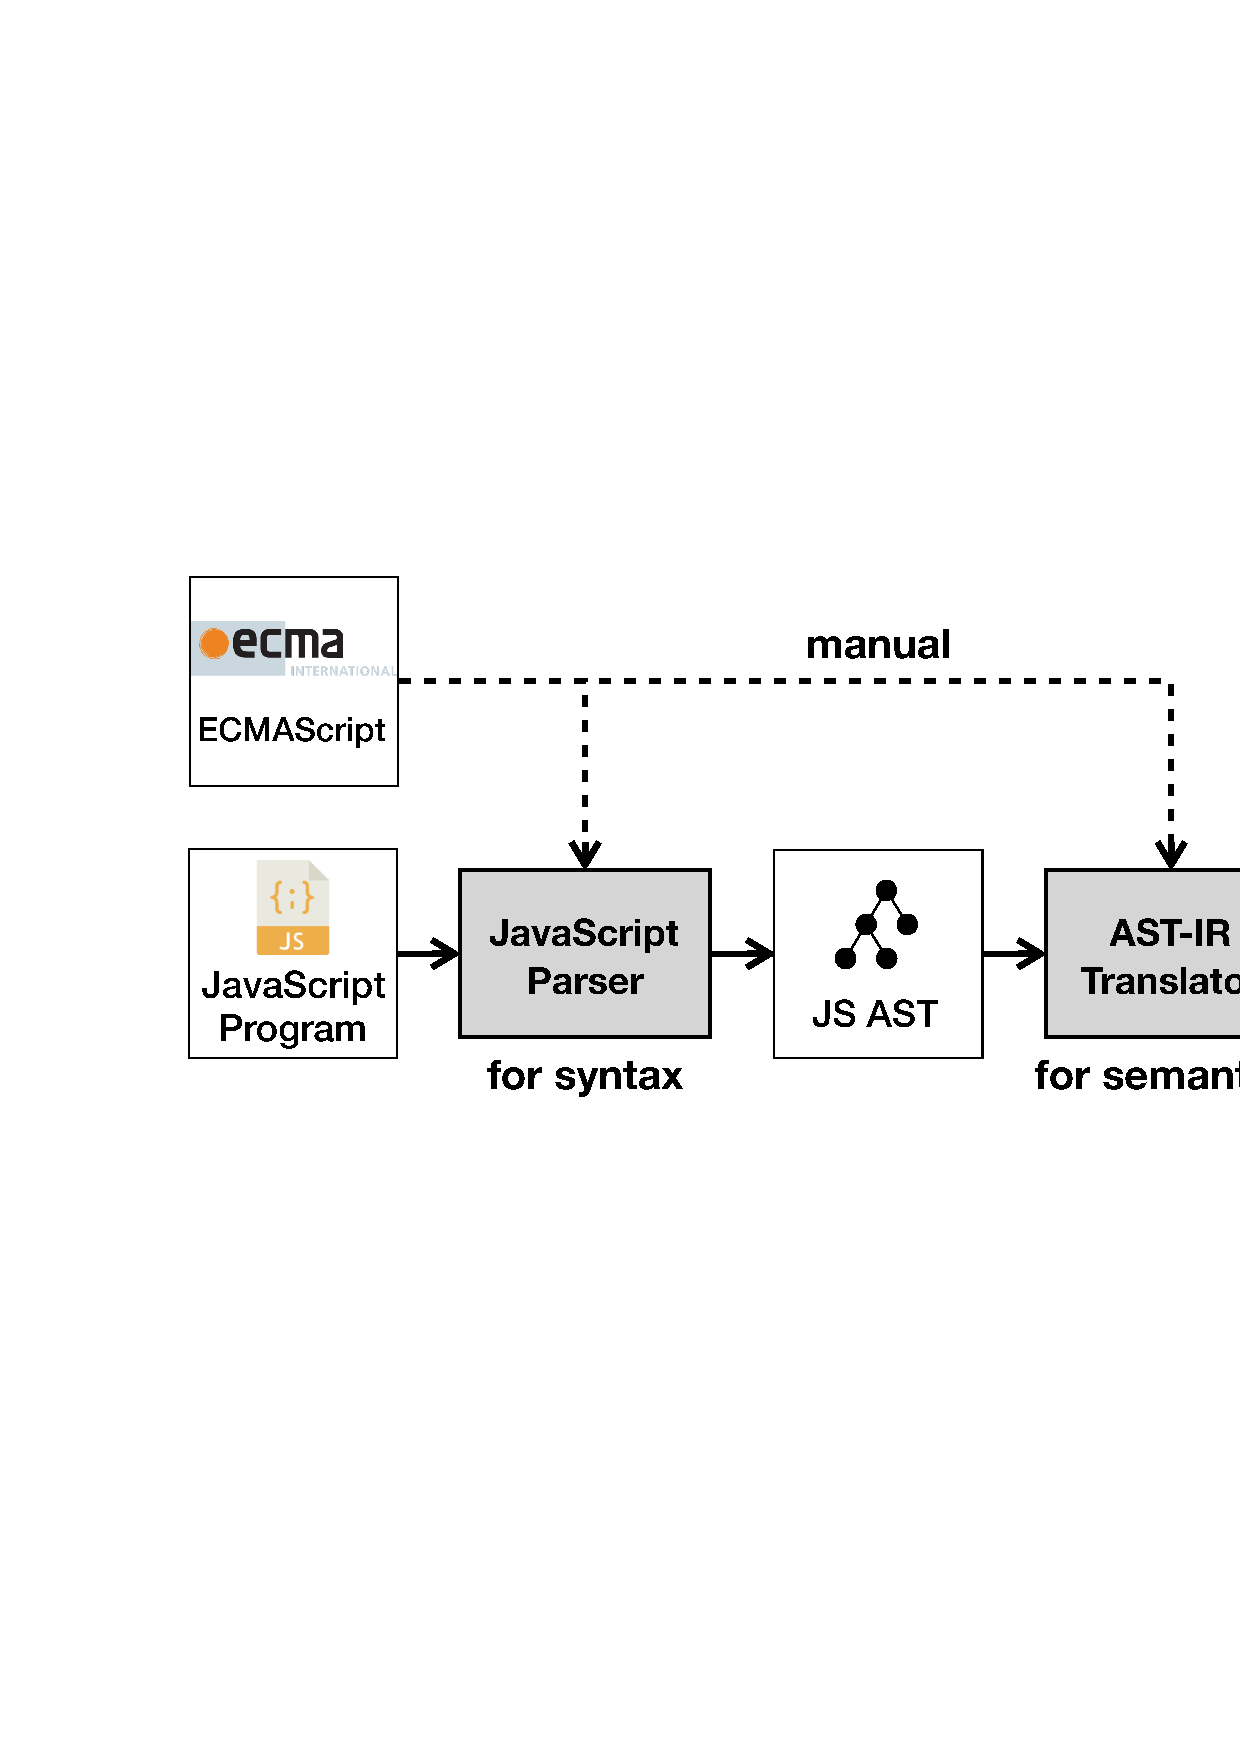
\includegraphics[width=0.48\textwidth]{img/existing.pdf}
\vspace*{-2em}
  \caption{Existing approaches: Manually built parsers and AST-IR
  translators for JavaScript IR-based semantics}
  \label{fig:existing}
\vspace*{-1em}
\end{figure}

Researchers have defined various JavaScript formal
semantics~\cite{aplas08,lambdajs,kjs,javert} suitable for static
analysis~\cite{jsai,tajs,wala,safe} and formal verification~\cite{javert} by
referring to ECMAScript.  ECMAScript is the official specification that
describes the JavaScript syntax using a variant of the extended BNF (EBNF) notation,
and its semantics using abstract algorithms written in English in a clear and
structured manner.  \textit{IR-based semantics extraction} is a traditional way to
define the formal semantics of a language by building a compiler front-end
that takes programs and produces their Intermediate
Representations (IRs) to indirectly represent the semantics of the given programs.
As illustrated in Figure~\ref{fig:existing}, a compiler front-end consists of a parser
that constructs Abstract Syntax Trees (ASTs) of given JavaScript programs, and
an AST-IR translator that converts ASTs to their own IRs.  It helps
researchers focus on IRs without worrying about diverse and enormous features of
JavaScript in developing new techniques for static analysis and formal
verification.

However, to the best of our knowledge, all existing approaches to JavaScript
IR-based semantics extraction \textit{manually} build parsers and translators.
Although manually building them was reasonable until ECMAScript 5.1 (ES5.1,
2011)~\cite{es5}, it is too tedious, labor-intensive, and
error-prone to deal with the large size of \textit{modern JavaScript} since ECMAScript 6
(ES6, 2015)~\cite{es6}. ES6 introduced numerous significantly new features such
as lexical binding via \( \code{let} \), the spread \( \code{...} \) operator,
classes, the \( \code{for-of} \) operator, the \( \code{async} \) functions, and
generators.  For example, consider KJS~\cite{kjs},
one of formal semantics of ES5.1 defined on top of \( \kframework \), which is
a framework for defining language semantics.
According to an author of KJS, it took
\textit{four months} to implement an AST-IR translator for 1,370 steps out of 2,932
steps in 368 abstract algorithms~\cite{kjsslides}. However, the most recent version of ECMAScript
(ES10, 2019)~\cite{es10} has 2,026 abstract algorithms consisting of 10,101
steps. Thus, the manual approaches do not seem to be scalable enough to build
an AST-IR translator for modern JavaScript,
and indeed no formal semantics exists for ES6 to ES10.

Moreover, JavaScript syntax and semantics are annually updated.  Until
ES5.1, JavaScript was a stable language because the specification was
rarely updated.  However, the Ecma Technical Committee 39 (TC39)~\cite{tc39}
decided to release the specification annually in late 2014.  After this official
announcement, several syntax features and roughly 1,000 to 3,000 steps of
abstract algorithms have been modified or newly added in the specification every year.
To handle these frequent and massive updates of ECMAScript,
the manual approaches require researchers to manually update parsers and AST-IR translators,
which incurs tremendous efforts.

To alleviate this problem, we propose a technique to \textit{automatically
synthesize} parsers and AST-IR translators directly from ECMAScript with
\textit{forward compatibility}. There are several technical challenges in
synthesizing parsers and translators. For syntax, ECMAScript utilizes its own
variant of EBNF with parametric non-terminals, conditional
alternatives, and various special terminal symbols.  Thus, no existing parser
generation technique is directly applicable for this variant.  Moreover,
JavaScript provides automatic semicolon insertion in its parsing algorithm with
several complex rules, not in a lexer. For semantics, abstract algorithms in
ECMAScript are written in English.  Besides, a general and forward compatible
representation of abstract algorithms is necessary to support future
versions of ECMAScript.

Our contribution is \( \tool \), a JavaScript IR-based Semantics Extraction
Toolchain:
\begin{itemize}[leftmargin=0.5cm]
  \item \textbf{\( \tool \) is the \textit{first tool that automatically
    extract} IR-based semantics from a language specification, ECMAScript.}
    For syntax, we formally introduce a variant of EBNF, \( \bnfes \),
    and propose a parser generation technique with
    lookahead parsing for \( \bnfes \), which supports automatic semicolon
    insertion. For semantics, we propose semi-automatic synthesis of AST-IR
    translators assisted by compile rules.  Compile rules describe
    how to convert each step of abstract algorithms into our intermediate
    representation \( \ires \) designed for ECMAScript. We evaluated \( \tool \)
    with the four most recent ECMAScript versions (ES7 to ES10).   \( \tool \)
    automatically generated parsers for all versions, and automatically compiled
    95.03\% of the steps in abstract algorithms on average.
  \item \textbf{\( \tool \) bridges gaps between the specification written in a
    natural language and tests.}
    To evaluate the correctness of \( \tool \), we checked the extracted
    semantics with the official test conformance suite, Test262~\cite{test262}.
    By manually completing missing parts of the AST-IR translator for the latest
    ECMAScript (ES10, 2019), we defined the \textit{first IR-based formal
    semantics of modern JavaScript}. It failed for 1,709 tests because of
    specification errors in ES10. Using the tests, we found eight specification errors,
    three of which had not been reported before. They were all confirmed by
    TC39 and will be fixed in the next release.  After fixing them, the formal
    semantics passed all 18,064 applicable tests.
  \item \textbf{\( \tool \) is also \textit{forward compatible} with new
    language features proposed for future ECMAScript specifications.}
    We evaluated the forward compatibility of \( \tool \) by applying it to all
    nine proposals that are ready for inclusion in the next ECMAScript
    (ES11, 2020).  It automatically synthesized parsers and compiled 560
    out of 595 algorithm steps for all the proposals.  After completion
    of the missing parts, we found three specifications errors in BigInt
    proposal by executing the corresponding tests in Test262.  After fixing
    them, the extracted semantics passed all applicable ES10 tests and 303 new
    applicable tests.
\end{itemize}
